\section{Kondisi Don't Care dan Implicant}

\subsection{Kondisi Don't Care}

Dalam praktik perancangan rangkaian digital, terdapat situasi di mana nilai output fungsi untuk kombinasi input tertentu tidak diperhatikan, baik karena kombinasi tersebut tidak mungkin terjadi secara fisik, maupun karena outputnya tidak memengaruhi operasi sistem secara keseluruhan. Kombinasi input semacam ini disebut \logic{kondisi don't care} dan dinotasikan dengan simbol $d$ atau $\times$ pada tabel kebenaran dan Peta Karnaugh \cite{rosen2019}.

\begin{definisi}[Kondisi Don't Care]
\logic{Kondisi don't care} adalah kombinasi input pada fungsi Boolean yang tidak memiliki spesifikasi output yang ditentukan. Perancang bebas menetapkan output 0 atau 1 untuk kondisi ini, bergantung pada pilihan mana yang menghasilkan penyederhanaan yang lebih optimal.
\end{definisi}

Contoh klasik kondisi don't care terdapat pada perancangan decoder BCD (\textit{Binary Coded Decimal}). Sistem BCD menggunakan 4 bit untuk merepresentasikan angka desimal 0 sampai 9, sehingga hanya menggunakan 10 dari 16 kemungkinan kombinasi 4-bit. Enam kombinasi sisanya ($1010$ sampai $1111$, yaitu desimal 10--15) tidak pernah muncul dalam operasi normal dan dapat dianggap sebagai don't care \cite{tutorialspoint_kmap}.

\subsection{Pemanfaatan Don't Care pada K-Map}

Pada Peta Karnaugh, sel-sel don't care diisi dengan simbol $\times$ (atau $d$). Saat membentuk kelompok, sel don't care dapat diperlakukan sebagai 1 jika penyertaannya memungkinkan pembentukan kelompok yang lebih besar, atau diabaikan (diperlakukan sebagai 0) jika tidak menguntungkan. Fleksibilitas ini memberikan kebebasan tambahan bagi perancang untuk menemukan ekspresi yang lebih sederhana.

\begin{contoh}
\textbf{K-Map dengan Don't Care}

Diberikan fungsi $F(A,B,C,D) = \sum m(1, 3, 7, 11, 15)$ dengan don't care $d(0, 2, 5)$.

\begin{center}
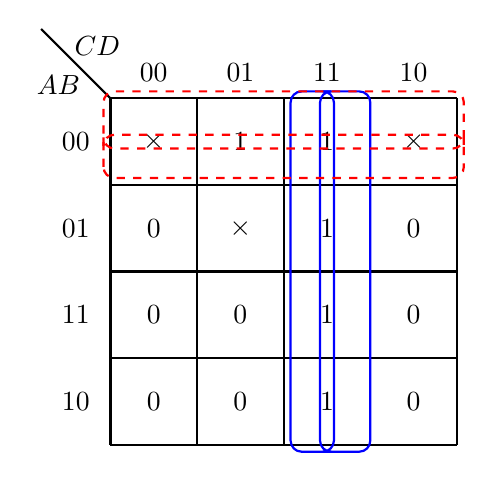
\begin{tikzpicture}[scale=1.1]
    \draw[thick] (0,0) grid (4,4);
    \draw[thick] (0,4) -- (-0.8,4.8);
    \node at (-0.6, 4.15) {$AB$};
    \node at (-0.15, 4.6) {$CD$};
    \node at (0.5, 4.3) {$00$}; \node at (1.5, 4.3) {$01$}; \node at (2.5, 4.3) {$11$}; \node at (3.5, 4.3) {$10$};
    \node at (-0.4, 3.5) {$00$}; \node at (-0.4, 2.5) {$01$}; \node at (-0.4, 1.5) {$11$}; \node at (-0.4, 0.5) {$10$};
    % Row 00: m0=d, m1=1, m3=1, m2=d
    \node at (0.5, 3.5) {$\times$}; \node at (1.5, 3.5) {1}; \node at (2.5, 3.5) {1}; \node at (3.5, 3.5) {$\times$};
    % Row 01: m4=0, m5=d, m7=1, m6=0
    \node at (0.5, 2.5) {0}; \node at (1.5, 2.5) {$\times$}; \node at (2.5, 2.5) {1}; \node at (3.5, 2.5) {0};
    % Row 11: m12=0, m13=0, m15=1, m14=0
    \node at (0.5, 1.5) {0}; \node at (1.5, 1.5) {0}; \node at (2.5, 1.5) {1}; \node at (3.5, 1.5) {0};
    % Row 10: m8=0, m9=0, m11=1, m10=0
    \node at (0.5, 0.5) {0}; \node at (1.5, 0.5) {0}; \node at (2.5, 0.5) {1}; \node at (3.5, 0.5) {0};
    % Group 1: column CD=11
    \draw[thick, blue, rounded corners] (2.42, -0.08) rectangle (2.58, 4.08);
    \draw[thick, blue, rounded corners] (2.08, -0.08) rectangle (3.0, 4.08);
    % Group 2: top row with don't cares
    \draw[thick, red, rounded corners, dashed] (-0.08, 3.42) rectangle (4.08, 3.58);
    \draw[thick, red, rounded corners, dashed] (-0.08, 3.08) rectangle (4.08, 4.08);
\end{tikzpicture}
\end{center}

Dengan memanfaatkan don't care:
\begin{itemize}
    \item \textcolor{blue}{Kelompok 1}: $\{m_3, m_7, m_{15}, m_{11}\}$ --- kolom $CD = 11$, seluruh sel bernilai 1, membentuk kelompok 4 sel $\Rightarrow$ suku: $CD$
    \item \textcolor{red}{Kelompok 2}: $\{m_0(\times), m_1, m_3, m_2(\times)\}$ --- baris $AB = 00$ dengan don't care, membentuk kelompok 4 sel $\Rightarrow$ suku: $A'B'$
\end{itemize}

\textbf{Hasil}: $F = CD + A'B'$

Tanpa don't care, ekspresi akan lebih panjang karena $m_1$ hanya bisa dikelompokkan sebagai pasangan, bukan kelompok 4.
\end{contoh}

\subsection{Prime Implicant dan Essential Prime Implicant}

\begin{definisi}[Prime Implicant]
Sebuah \logic{prime implicant} adalah kelompok sel bernilai 1 (dan opsional don't care) pada K-Map yang bersifat \textbf{maksimal}, yaitu tidak dapat diperbesar lagi tanpa menyertakan sel yang bernilai 0. Setiap prime implicant merepresentasikan suku perkalian yang paling sederhana yang masih merupakan implikan dari fungsi \cite{rosen2019}.
\end{definisi}

\begin{definisi}[Essential Prime Implicant]
Sebuah \logic{essential prime implicant} adalah prime implicant yang mencakup setidaknya satu sel bernilai 1 yang \textbf{tidak dicakup} oleh prime implicant lainnya. Essential prime implicant \textbf{wajib} disertakan dalam ekspresi akhir, karena tanpanya terdapat minterm yang tidak terwakili.
\end{definisi}

Prosedur sistematis untuk menemukan ekspresi minimal menggunakan K-Map adalah sebagai berikut:

\begin{enumerate}
  \item Identifikasi semua prime implicant pada K-Map.
  \item Tentukan essential prime implicant --- yaitu prime implicant yang mencakup minterm yang tidak dicakup oleh prime implicant lainnya.
  \item Sertakan semua essential prime implicant dalam ekspresi akhir.
  \item Jika masih terdapat minterm yang belum tercakup, pilih prime implicant tambahan yang mencakup sisa minterm dengan jumlah suku seminimal mungkin.
\end{enumerate}

\begin{catatan}
Membedakan prime implicant dari non-prime implicant adalah keterampilan penting. Kelompok yang bukan prime implicant selalu dapat diperbesar menjadi kelompok yang lebih besar (prime implicant), sehingga tidak perlu dipertimbangkan dalam solusi akhir.
\end{catatan}
